\chapter{Preliminary results using pseudodata}\label{ch:appendix_pseudodata}

CMS Collaboration papers go through a series of steps summarized in Fig.~\ref{Fig:CMSPubJourney} before they get submitted to a journal. 
When an analysis has reached a certain maturity, the Physics Working group and the analyzers make sure that the simulations had taken into account detector malfunctions/resolution in the preliminary conclusions, the physics working group greenlights the project for ``unblinding" in the preapproval stage. Prior to this stage, the analysis results remained blinded for $\mgg$ above 1 TeV. In lieu of the real CMS data, pseudodata have been generated to test and validate our prediction. 

\begin{figure}[h!]\centering
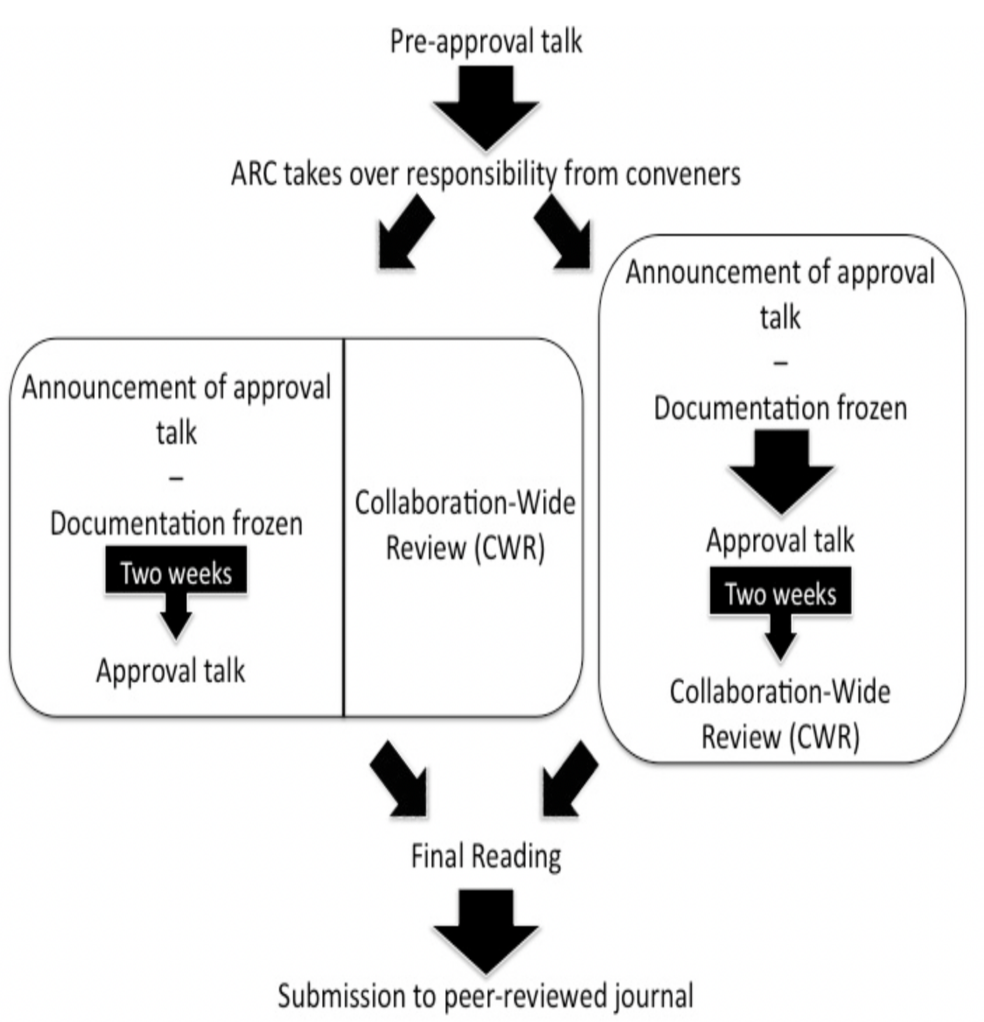
\includegraphics[scale=0.7]{fig/CMSPublication.png}
\caption{CMS Collaboration papers go pre-approval, approval, a Collaboration-Wide Review, and a final reading prior to submission to a peer-reviewed journal~\cite{CMSPublishing}.}
\label{Fig:CMSPubJourney}
\end{figure}


The pseudodata have been generated using the sum of the $\gamma+\gamma \textnormal{j}+jj$ spectra or what we call the prefit background estimate. For each bin, a poisson distribution with a mean equal to the prefit value, is used to generate random integer yields. In this way, the pseudodata feature realistic systematic structures and fluctuations. Thus, we can check whether prefit trends in pulls are covered by the current parametrization. 

%%%%%% REPLACING DATA BY PSEUDODATA 
\begin{figure}[!htbp]{\centering{
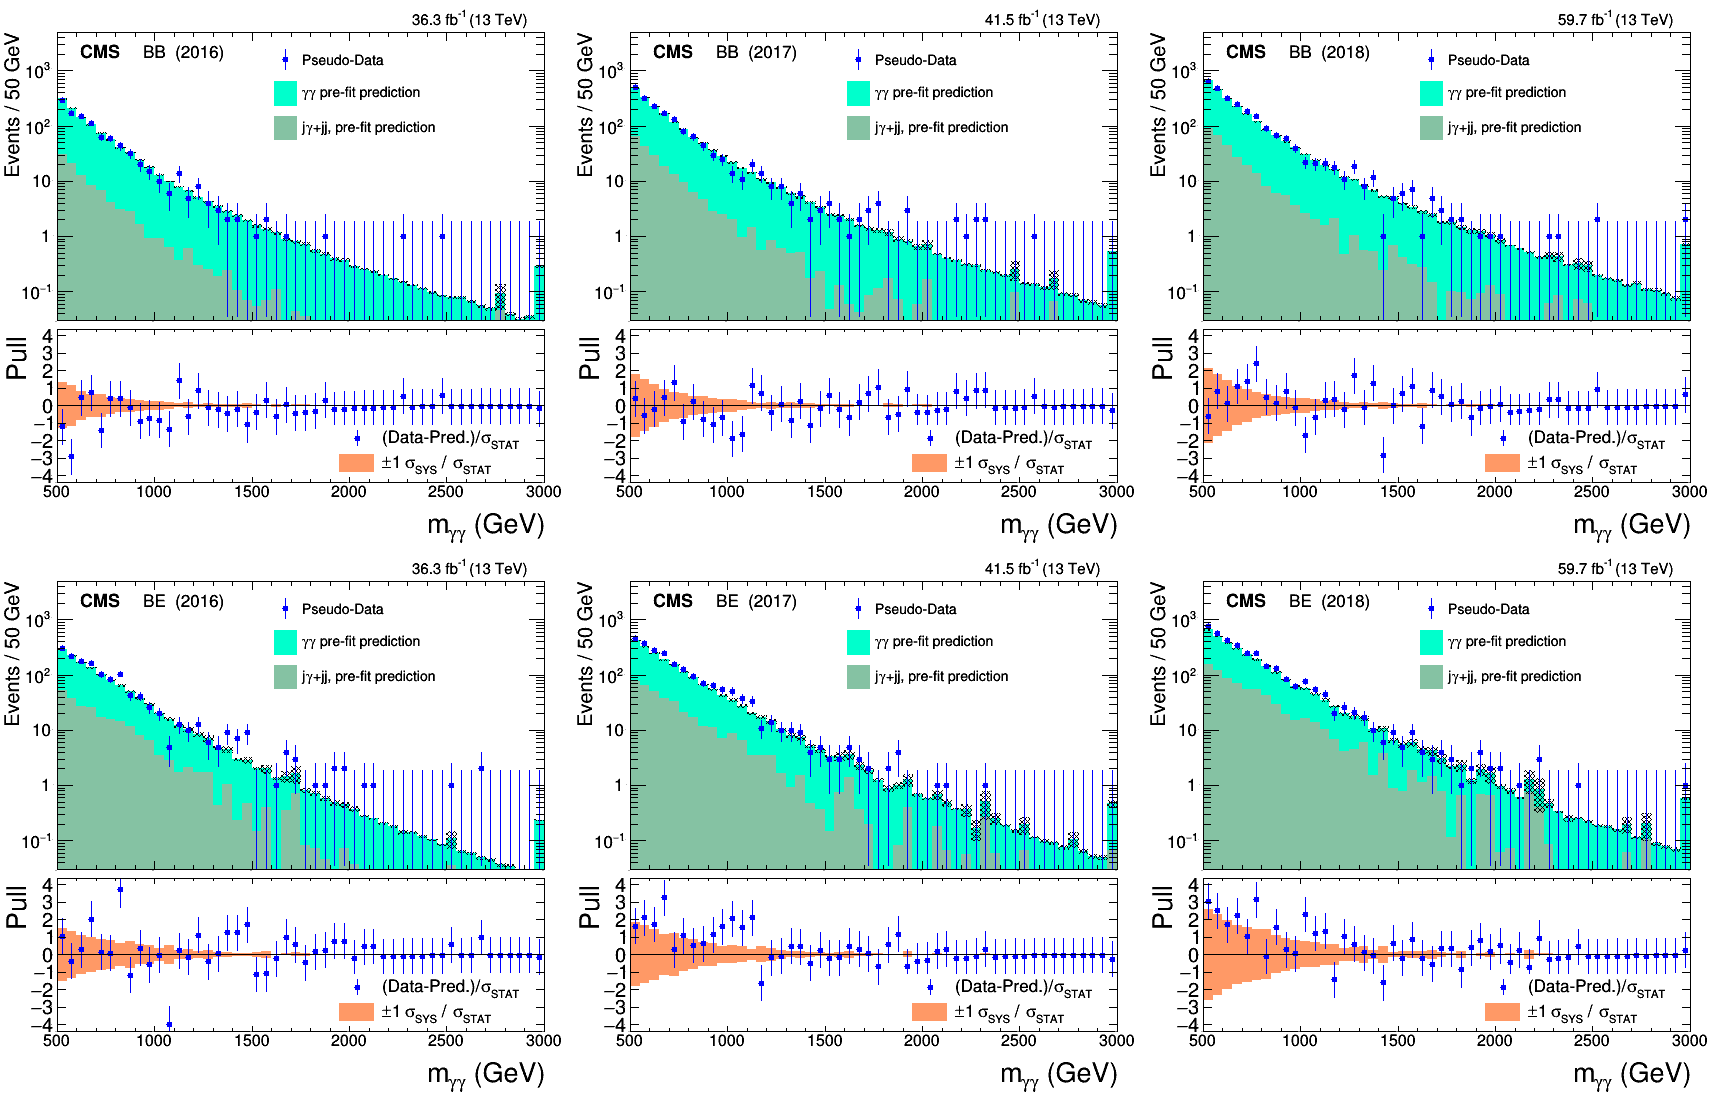
\includegraphics[width=1.0\textwidth]{fig/PRED_PRE_ADDGRW.png}
%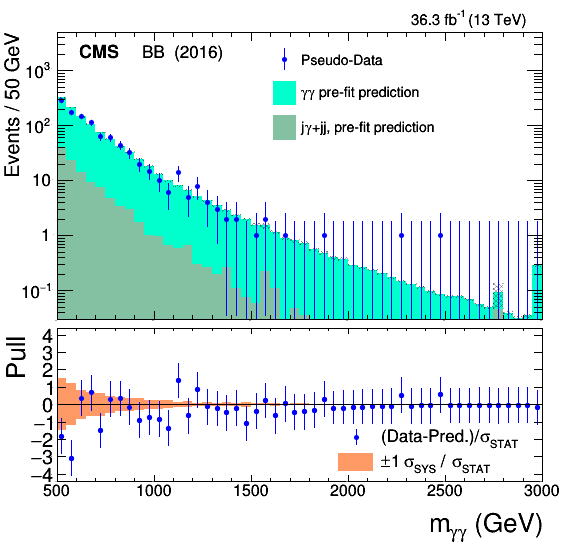
\includegraphics[width=0.49\textwidth]{fig/PLOT_PRED_PULL_BB16_0_1.png}
%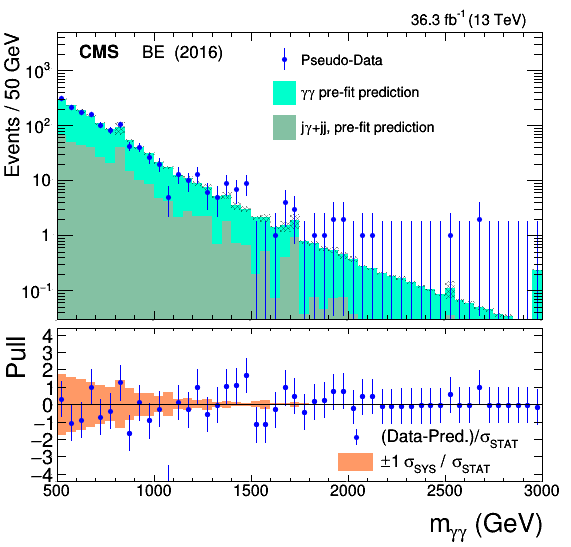
\includegraphics[width=0.49\textwidth]{fig/PLOT_PRED_PULL_BE16_0_1.png}
%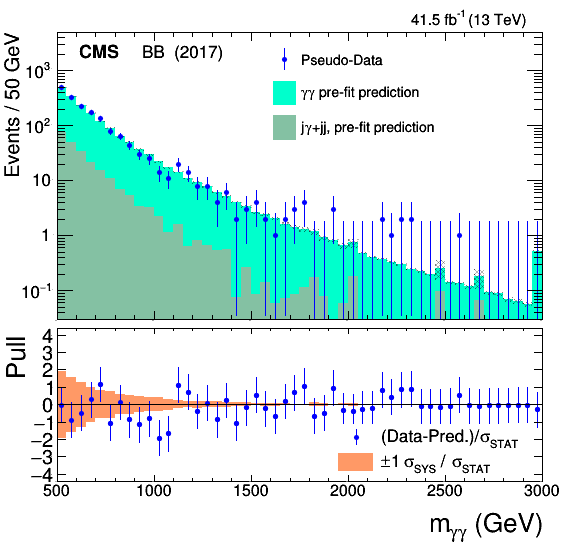
\includegraphics[width=0.49\textwidth]{fig/PLOT_PRED_PULL_BB17_0_1.png}
%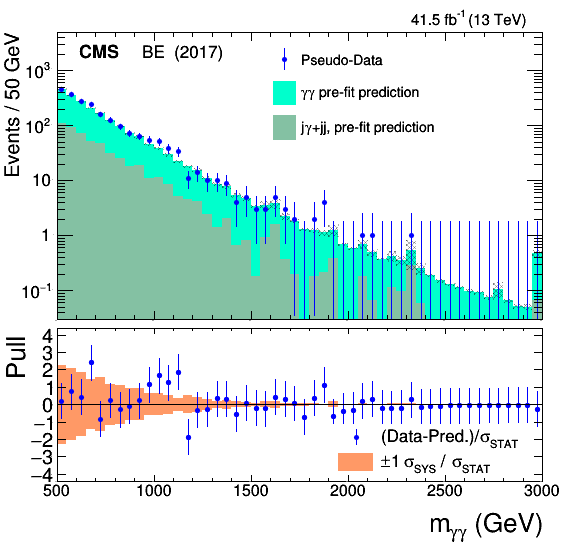
\includegraphics[width=0.49\textwidth]{fig/PLOT_PRED_PULL_BE17_0_1.png}
%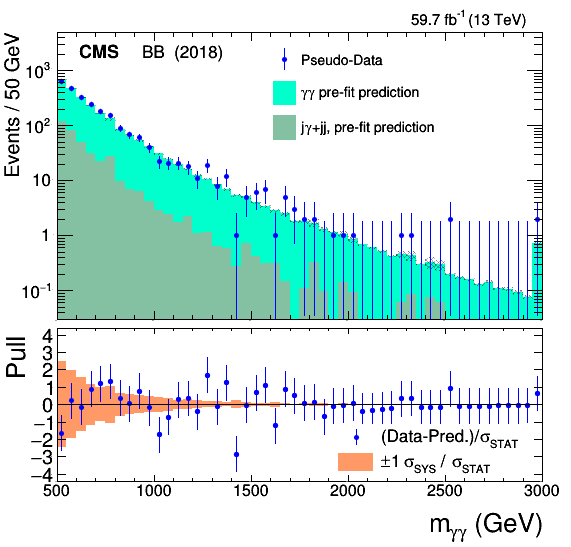
\includegraphics[width=0.49\textwidth]{fig/PLOT_PRED_PULL_BB18_0_1.png}
%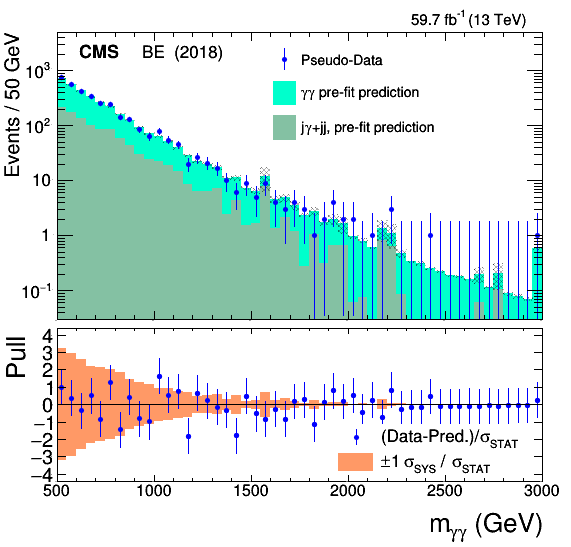
\includegraphics[width=0.49\textwidth]{fig/PLOT_PRED_PULL_BE18_0_1.png}}
\caption{The prefit spectra with the generated pseudodata for BB (top) and BE (bottom) for the tree years of data taking (left to right: 2016, 2017, 2018).}
\label{fig:Prefit_Pseudo}}
\end{figure}

For the limit setting, the \mgg spectra shown in Fig.~\ref{fig:Prefit_Pseudo} are used. The six \mgg spectra are binned in 100 GeV sizes, starting at 500 \GeV and ending at 4000 \GeV. Last bin contains the overflow above 4000 \GeV. 

\subsection{Clockwork Results with Pseudodata}

For the Continuum Clockwork model, we start the fit from 1 \TeV as we are constrained by the available ADD samples. Below this, statistical fluctuations are too high to arrive at any meaningful conclusions. In running \THETA, the nuisance parameters are simultaneously marginalized in a bayesian marginalization constrain fit, and a posterior prediction for the combined diphoton+fake \mgg spectra produced using the pseudodata as the constraint. The signal strength is given a flat prior bounded below by zero, although the background normalization is allowed to float freely (within 5\%). This approach presupposes that the signal and background differ in their shape and not only in the rate. A benefit from the shape-based analysis is that we are able to absorb higher-order corrections to the diphoton prediction that are (in principle) unknown directly into the background model under the assumption that those higher-order corrections resulted in a relatively flat k-factor. 

The bayesian marginalization gives out the postfit results which are presented in Fig.~\ref{Fig:Postfit_mgg_Clockwork_pseudo}. The bottom pads show that the pulls or the various systematic trends initially present in the prefit pulls are smoothened out in the postfit version. For pseudodata, the origin of these trends is random and arbitrary. The pseudodata happened to deviate in the same direction for a few sequential bins. The postfit pulls exhibit only statistical fluctuations around one, and thus the \mgg parametrization absorbs the systematic effects. 

 

\begin{figure}[h!]\centering
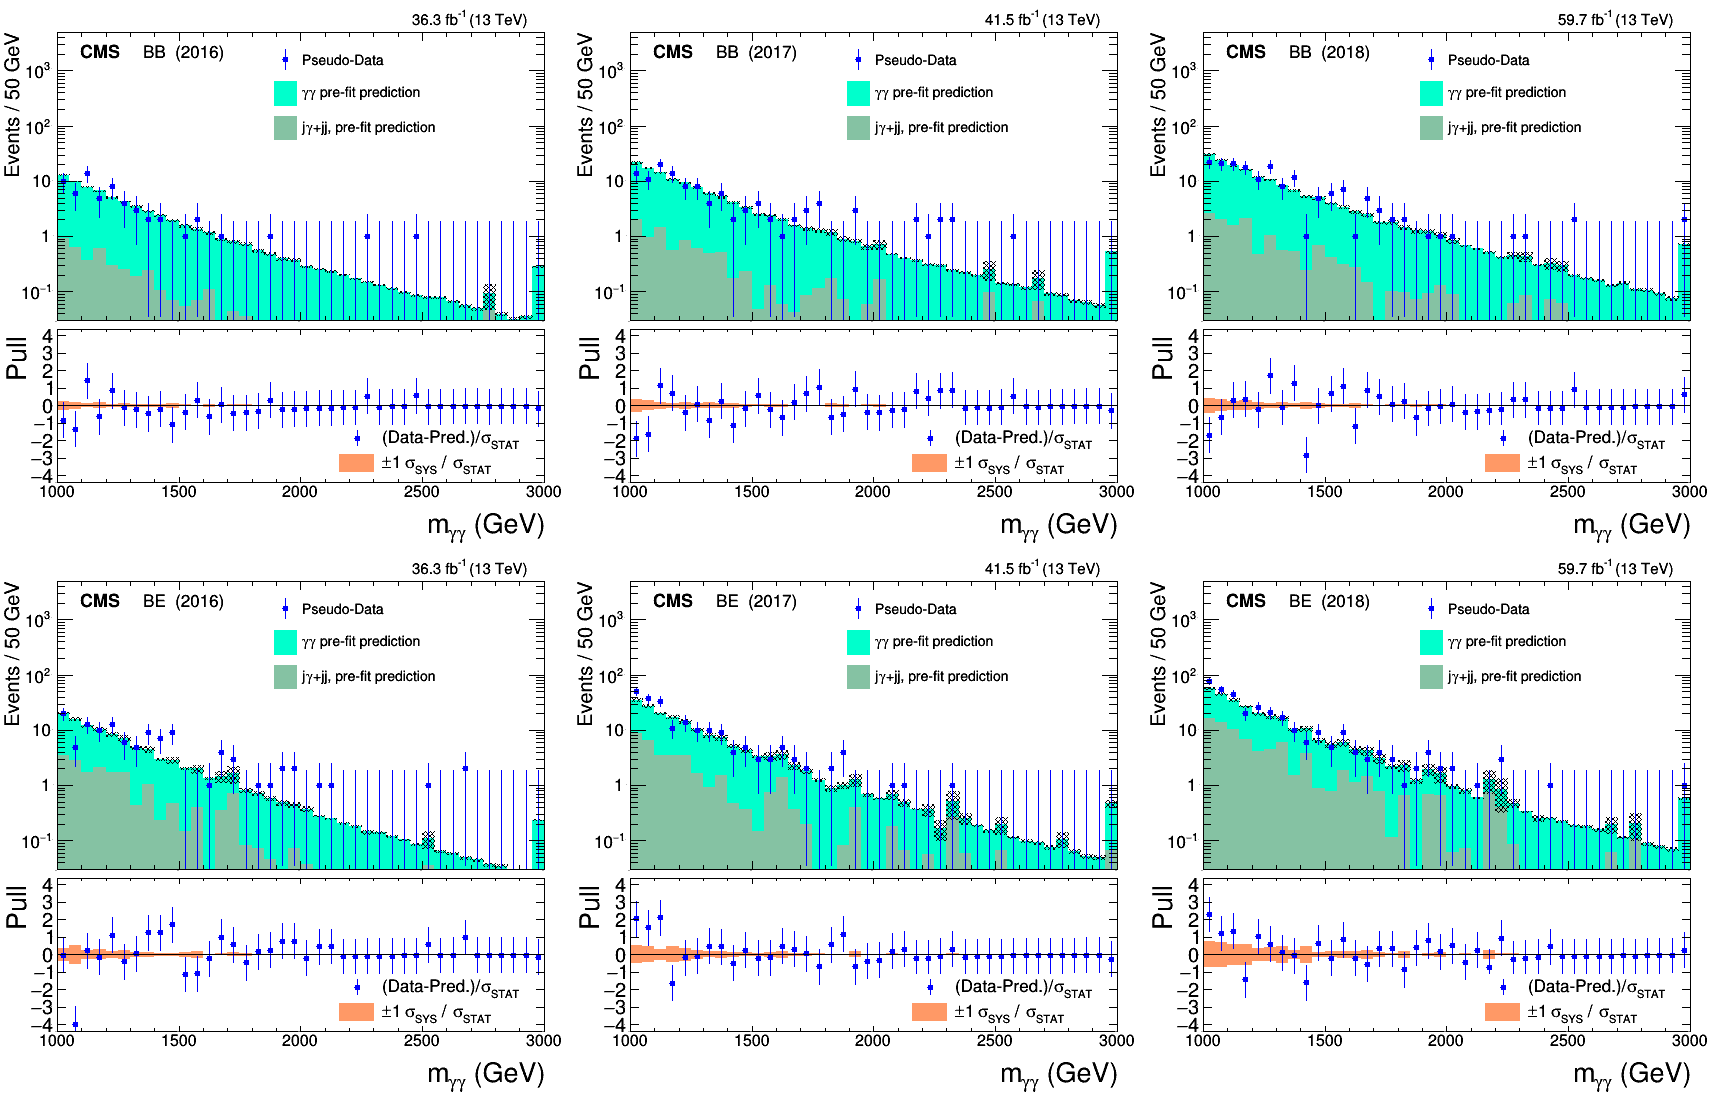
\includegraphics[width=1.\linewidth]{fig/PRED_PRE_CWk.png}
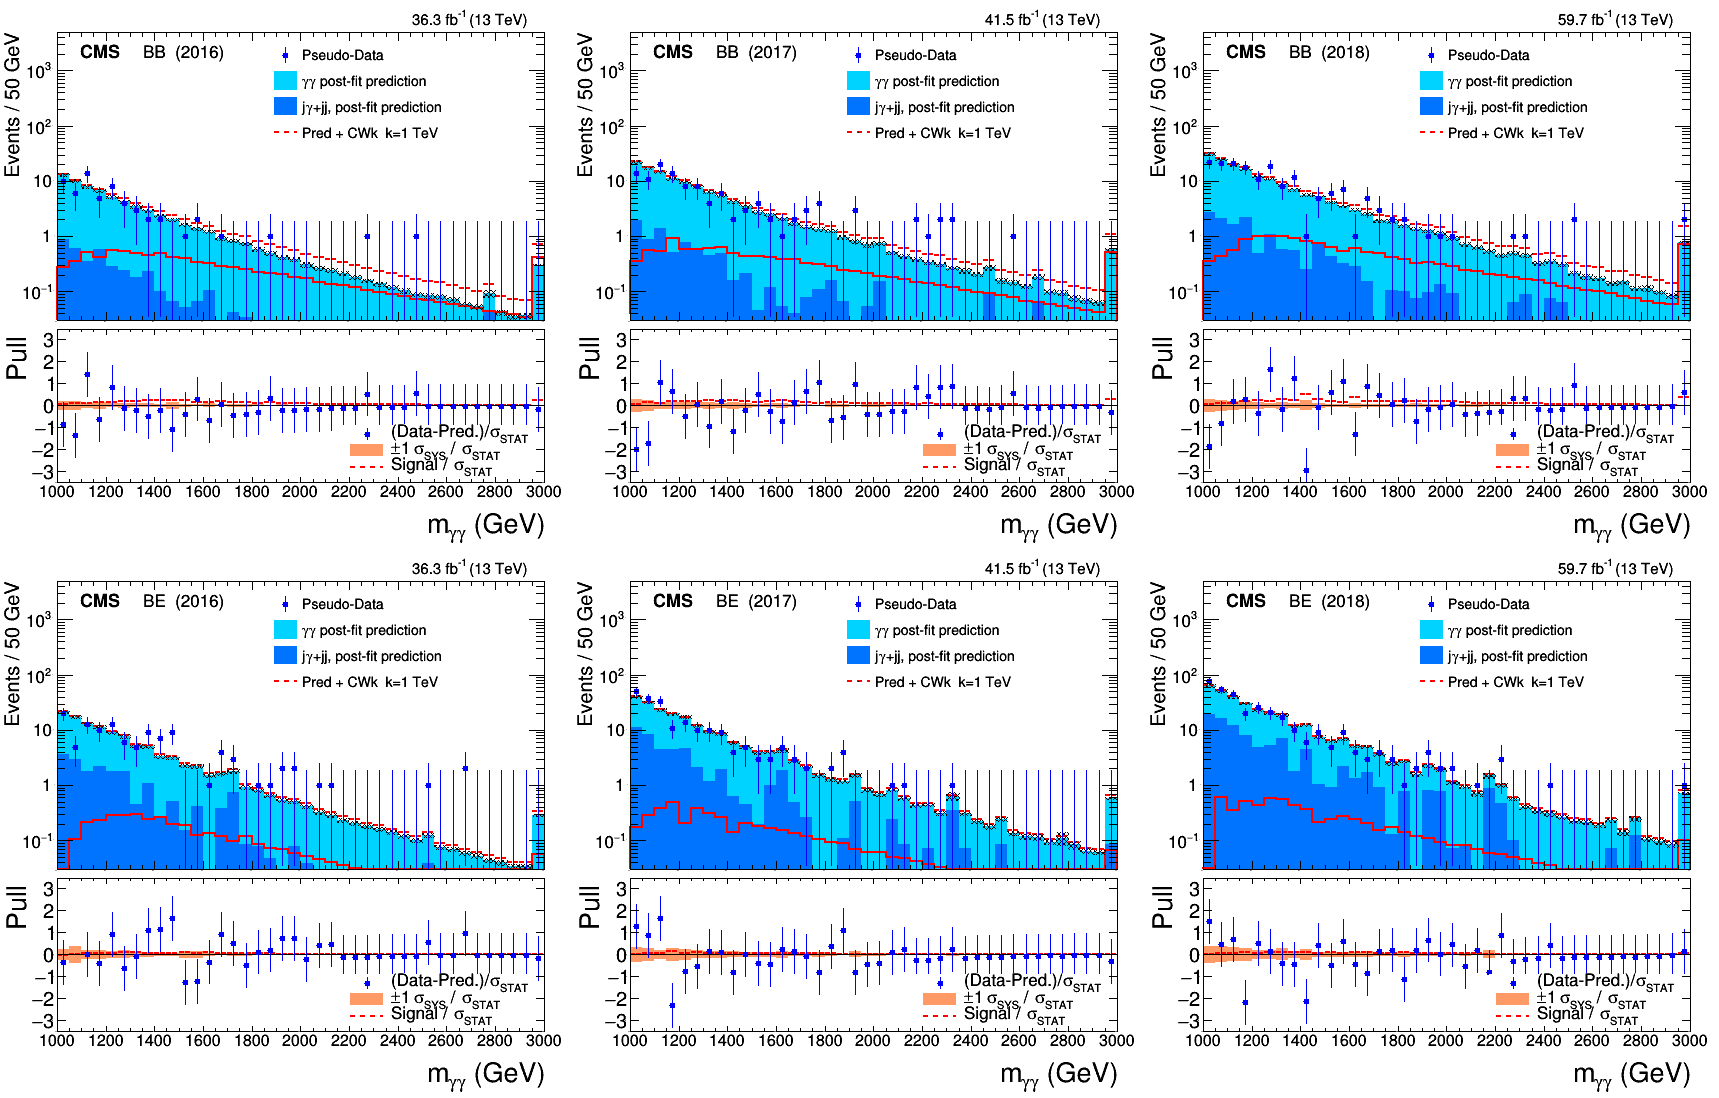
\includegraphics[width=1.\linewidth]{fig/PRED_POST_CWk.png}
\caption{The prefit (top two rows) and the postfit (bottom two rows) \mgg spectra for the Clockwork Model using pseudodata.
Columns left to right correspond to the years 2016, 2017, and 2018 respectively.}
\label{Fig:Postfit_mgg_Clockwork_pseudo}
\end{figure}

In this portion, we make additional commentaries on the nuisance parameters considered in the marginalization procedure. In Fig.~\ref{Fig:Postfit_mgg_Clockwork_pseudo}, we see that the signal strength $\beta$, named as \texttt{beta\_signal}, shown in the top left is strongly constrained near zero as expected. Normalization nuisances of real $\gamma\gamma$ and fake background events are  constrained and their postfit pdfs are close to zero some value dictated by the fit on pseudodata. Figures~\ref{fig:Postfit_NuisancesPDFs} and ~\ref{fig:Postfit_NuisancesPDFs2}, correspond to the 50 pdfs of the PDF nuisances. They are all close to the prefit and appear as a gaussian with mean zero and standard deviation of one as this set of pseudodata cannot constrain them further.

Note here that the nuisances are constrained and their priors which are either gaussian or lognormal probability distribution functions transform into their corresponding postfit versions. While \COMBINE, provides summary tables with the means and the standard deviations of the nuisances postfit pdfs, \THETA provides the full postfit pdf spectra of each nuisance. Overall, the postfit results suggest a healthy performance of the limit code and fit procedure which will be used in the actual data. Finally, Fig.~\ref{Fig:LIMIT_Clockwork} shows a comparable shape trend with the 2016 result~\cite{cmsdiphoton2016} which is shown in Fig.~\ref{fig:ClockworkCMS2016}.




\begin{figure}[!htbp]{\centering{
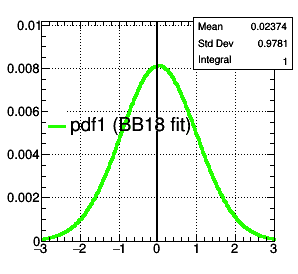
\includegraphics[width=0.16\textwidth]{fig/posteriors__pdf1_BB18_fitBBBE161718_ADDGRW.png}
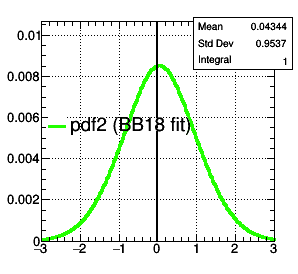
\includegraphics[width=0.16\textwidth]{fig/posteriors__pdf2_BB18_fitBBBE161718_ADDGRW.png}
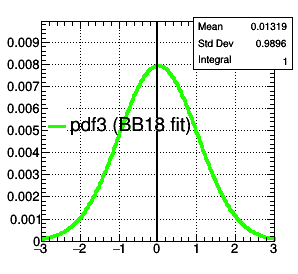
\includegraphics[width=0.16\textwidth]{fig/posteriors__pdf3_BB18_fitBBBE161718_ADDGRW.png}
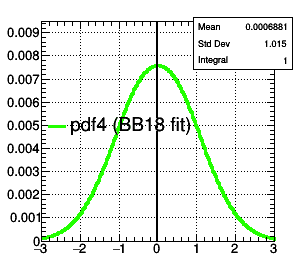
\includegraphics[width=0.16\textwidth]{fig/posteriors__pdf4_BB18_fitBBBE161718_ADDGRW.png}
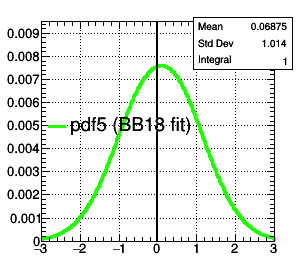
\includegraphics[width=0.16\textwidth]{fig/posteriors__pdf5_BB18_fitBBBE161718_ADDGRW.png}\\
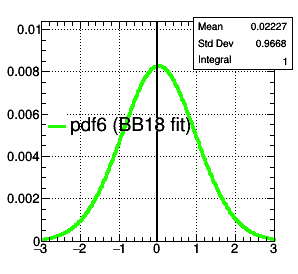
\includegraphics[width=0.16\textwidth]{fig/posteriors__pdf6_BB18_fitBBBE161718_ADDGRW.png}
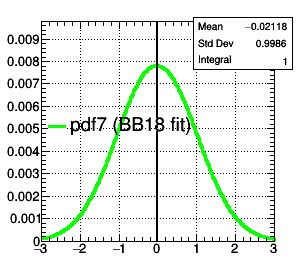
\includegraphics[width=0.16\textwidth]{fig/posteriors__pdf7_BB18_fitBBBE161718_ADDGRW.png}
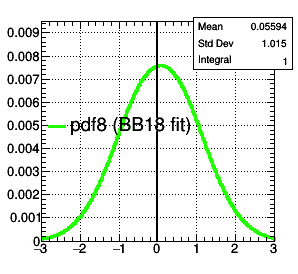
\includegraphics[width=0.16\textwidth]{fig/posteriors__pdf8_BB18_fitBBBE161718_ADDGRW.png}
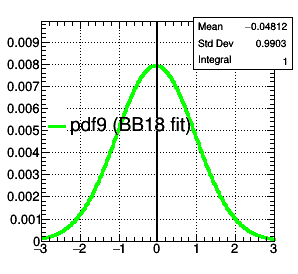
\includegraphics[width=0.16\textwidth]{fig/posteriors__pdf9_BB18_fitBBBE161718_ADDGRW.png}
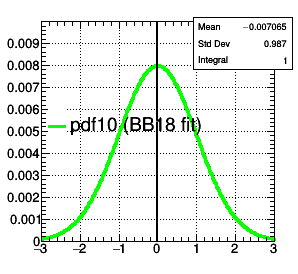
\includegraphics[width=0.16\textwidth]{fig/posteriors__pdf10_BB18_fitBBBE161718_ADDGRW.png}\\
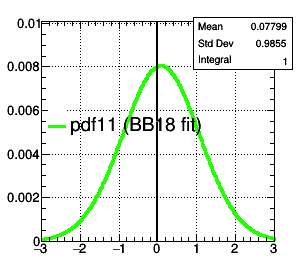
\includegraphics[width=0.16\textwidth]{fig/posteriors__pdf11_BB18_fitBBBE161718_ADDGRW.png}
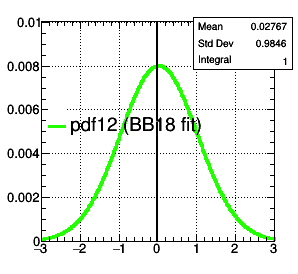
\includegraphics[width=0.16\textwidth]{fig/posteriors__pdf12_BB18_fitBBBE161718_ADDGRW.png}
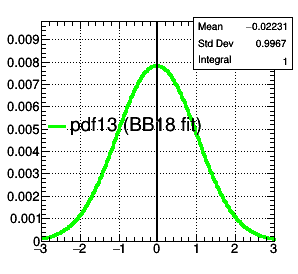
\includegraphics[width=0.16\textwidth]{fig/posteriors__pdf13_BB18_fitBBBE161718_ADDGRW.png}
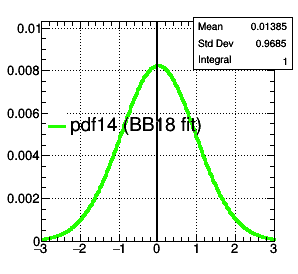
\includegraphics[width=0.16\textwidth]{fig/posteriors__pdf14_BB18_fitBBBE161718_ADDGRW.png}
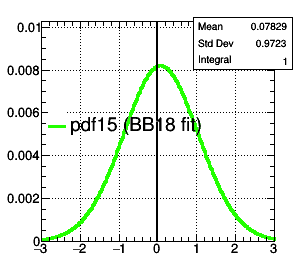
\includegraphics[width=0.16\textwidth]{fig/posteriors__pdf15_BB18_fitBBBE161718_ADDGRW.png}\\
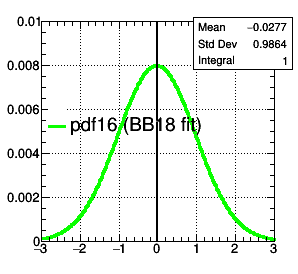
\includegraphics[width=0.16\textwidth]{fig/posteriors__pdf16_BB18_fitBBBE161718_ADDGRW.png}
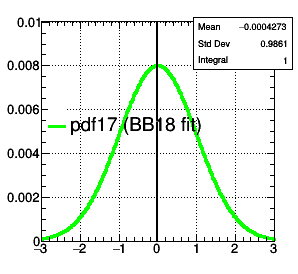
\includegraphics[width=0.16\textwidth]{fig/posteriors__pdf17_BB18_fitBBBE161718_ADDGRW.png}
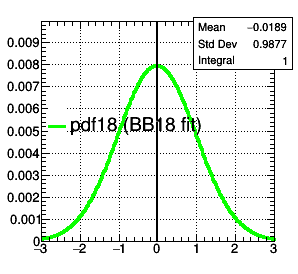
\includegraphics[width=0.16\textwidth]{fig/posteriors__pdf18_BB18_fitBBBE161718_ADDGRW.png}
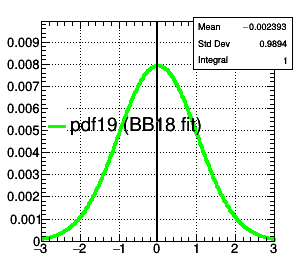
\includegraphics[width=0.16\textwidth]{fig/posteriors__pdf19_BB18_fitBBBE161718_ADDGRW.png}
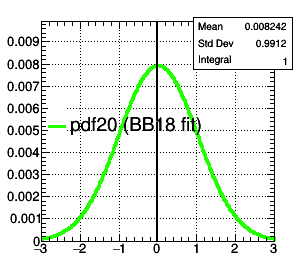
\includegraphics[width=0.16\textwidth]{fig/posteriors__pdf20_BB18_fitBBBE161718_ADDGRW.png}\\
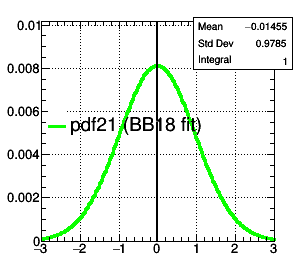
\includegraphics[width=0.16\textwidth]{fig/posteriors__pdf21_BB18_fitBBBE161718_ADDGRW.png}
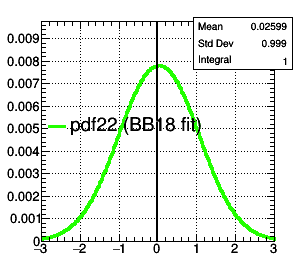
\includegraphics[width=0.16\textwidth]{fig/posteriors__pdf22_BB18_fitBBBE161718_ADDGRW.png}
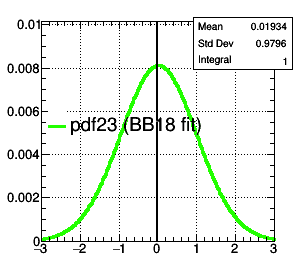
\includegraphics[width=0.16\textwidth]{fig/posteriors__pdf23_BB18_fitBBBE161718_ADDGRW.png}
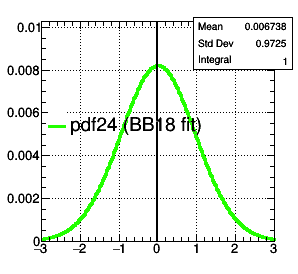
\includegraphics[width=0.16\textwidth]{fig/posteriors__pdf24_BB18_fitBBBE161718_ADDGRW.png}
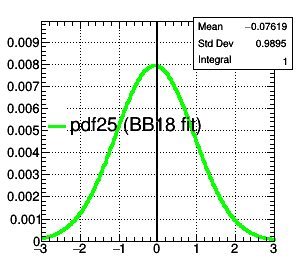
\includegraphics[width=0.16\textwidth]{fig/posteriors__pdf25_BB18_fitBBBE161718_ADDGRW.png}\\
\caption{The postfit probability distribution functions (pdfs) for the first 25 nuisances of the parton distribution functions (PDFs) in the six-SRs fit.The statistics panel displays the mean and the std of each pdf. This set of results corresponds to the pseudodata.}
\label{fig:Postfit_NuisancesPDFs}
\end{figure}

% This set of postfit pdfs complements the one shown in fig. ~\ref{fig:Postfit_Nuisances} and fig.~\ref{fig:Postfit_Nuisances2} .


\begin{figure}[!htbp]{\centering{
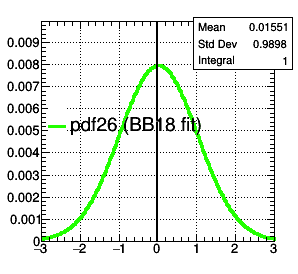
\includegraphics[width=0.16\textwidth]{fig/posteriors__pdf26_BB18_fitBBBE161718_ADDGRW.png}
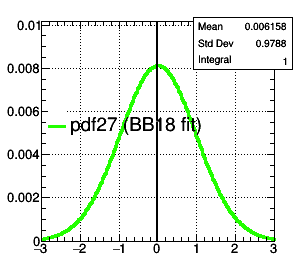
\includegraphics[width=0.16\textwidth]{fig/posteriors__pdf27_BB18_fitBBBE161718_ADDGRW.png}
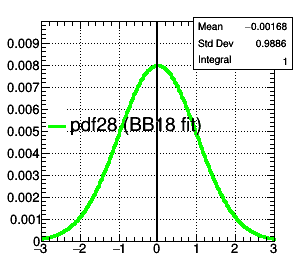
\includegraphics[width=0.16\textwidth]{fig/posteriors__pdf28_BB18_fitBBBE161718_ADDGRW.png}
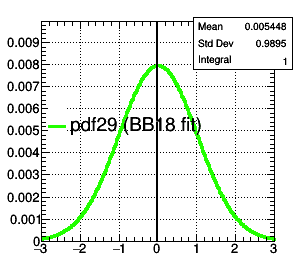
\includegraphics[width=0.16\textwidth]{fig/posteriors__pdf29_BB18_fitBBBE161718_ADDGRW.png}
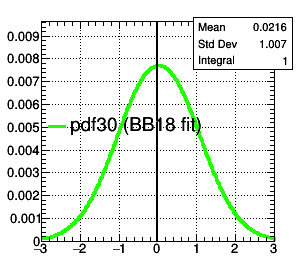
\includegraphics[width=0.16\textwidth]{fig/posteriors__pdf30_BB18_fitBBBE161718_ADDGRW.png}\\
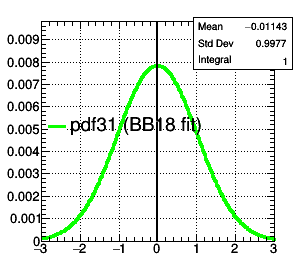
\includegraphics[width=0.16\textwidth]{fig/posteriors__pdf31_BB18_fitBBBE161718_ADDGRW.png}
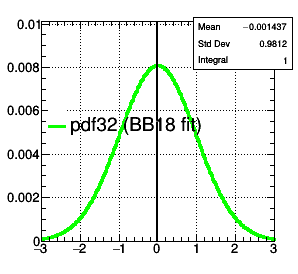
\includegraphics[width=0.16\textwidth]{fig/posteriors__pdf32_BB18_fitBBBE161718_ADDGRW.png}
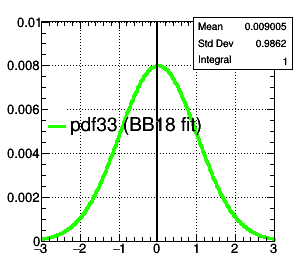
\includegraphics[width=0.16\textwidth]{fig/posteriors__pdf33_BB18_fitBBBE161718_ADDGRW.png}
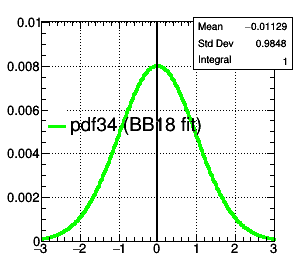
\includegraphics[width=0.16\textwidth]{fig/posteriors__pdf34_BB18_fitBBBE161718_ADDGRW.png}
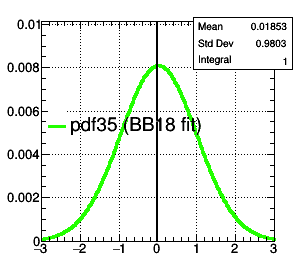
\includegraphics[width=0.16\textwidth]{fig/posteriors__pdf35_BB18_fitBBBE161718_ADDGRW.png}\\
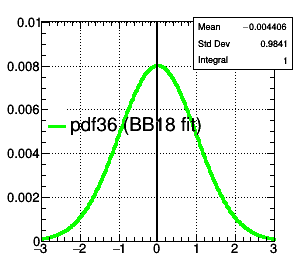
\includegraphics[width=0.16\textwidth]{fig/posteriors__pdf36_BB18_fitBBBE161718_ADDGRW.png}
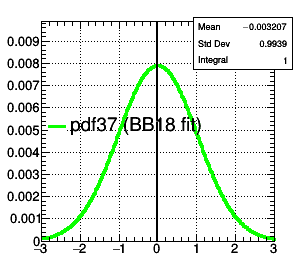
\includegraphics[width=0.16\textwidth]{fig/posteriors__pdf37_BB18_fitBBBE161718_ADDGRW.png}
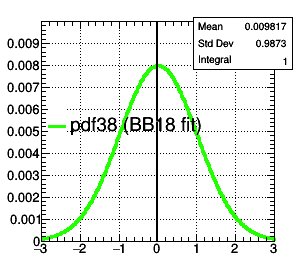
\includegraphics[width=0.16\textwidth]{fig/posteriors__pdf38_BB18_fitBBBE161718_ADDGRW.png}
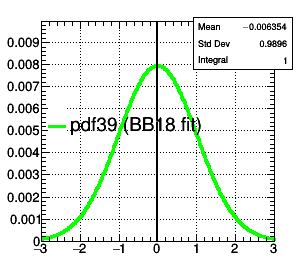
\includegraphics[width=0.16\textwidth]{fig/posteriors__pdf39_BB18_fitBBBE161718_ADDGRW.png}
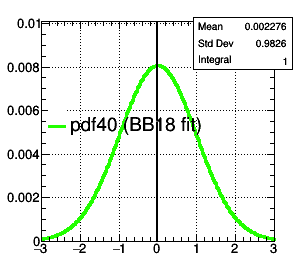
\includegraphics[width=0.16\textwidth]{fig/posteriors__pdf40_BB18_fitBBBE161718_ADDGRW.png}\\
\includegraphics[width=0.16\textwidth]{fig/posteriors__pdf41_BB18_fitBBBE161718_ADDGRW.png}
\includegraphics[width=0.16\textwidth]{fig/posteriors__pdf42_BB18_fitBBBE161718_ADDGRW.png}
\includegraphics[width=0.16\textwidth]{fig/posteriors__pdf43_BB18_fitBBBE161718_ADDGRW.png}
\includegraphics[width=0.16\textwidth]{fig/posteriors__pdf44_BB18_fitBBBE161718_ADDGRW.png}
\includegraphics[width=0.16\textwidth]{fig/posteriors__pdf45_BB18_fitBBBE161718_ADDGRW.png}\\
\includegraphics[width=0.16\textwidth]{fig/posteriors__pdf46_BB18_fitBBBE161718_ADDGRW.png}
\includegraphics[width=0.16\textwidth]{fig/posteriors__pdf47_BB18_fitBBBE161718_ADDGRW.png}
\includegraphics[width=0.16\textwidth]{fig/posteriors__pdf48_BB18_fitBBBE161718_ADDGRW.png}
\includegraphics[width=0.16\textwidth]{fig/posteriors__pdf49_BB18_fitBBBE161718_ADDGRW.png}
\includegraphics[width=0.16\textwidth]{fig/posteriors__pdf50_BB18_fitBBBE161718_ADDGRW.png} }
\caption{The postfit probability distribution functions (pdfs) for the last 25 nuisances of the parton distribution functions (PDFs) in the six-SRs fit. The statistics panel displays the mean and the std of each pdf.
This set of results corresponds to the pseudodata.}
\label{fig:Postfit_NuisancesPDFs2}
\end{figure}

% This set of postfit pdfs complements the one shown in fig. \ref{fig:Postfit_Nuisances26_50}.



\begin{figure}[h!]\centering
\includegraphics[width=1.\linewidth]{fig/POST_All_BBBE161718_CWk.png}
\caption{The postfit pdfs for the 25 nuisance parameters used in the six SRs fit with CW model signal using pseudodata.
(We omit the illustration of the other 50 of PDFs pdfs as they are gaussian-like without particular interest.)}
}
\label{Fig:Postift_Nuisances_Clockwork}
\end{figure}

%%%%%%%%%%%%% POSTFIT RESULTS USING PSEUDODATA 
\begin{figure}[h!]\centering
\includegraphics[width=0.49\linewidth]{fig/LIMITPLOT_BBBE161718_CWk.png}
\includegraphics[width=0.47\linewidth]{fig/LIMITPLOT_BBBE161718_CWk_nonLog.png}
\caption{The exclusion limit for the continuous graviton model in the clockwork framework over the $k-M_5$ parameter space using pseudodata.
The shaded region denotes where the theory becomes non-perturbative.
(The right plots is the same as the left one but in non-log axis).
The result from the fit over all six SRs (collectively over all years and channels).}
\label{Fig:LIMIT_Clockwork}
\end{figure}

\subsection{ADD Results with Pseudodata}

For want of space, we exclude the pseudodata results for the ADD. But the procedure is the same as that for the Clockwork model except we begin below 1~\TeV.